\documentclass[tikz,border=8pt]{standalone}
\usepackage{amsmath}
\usetikzlibrary{arrows.meta,positioning}

\begin{document}
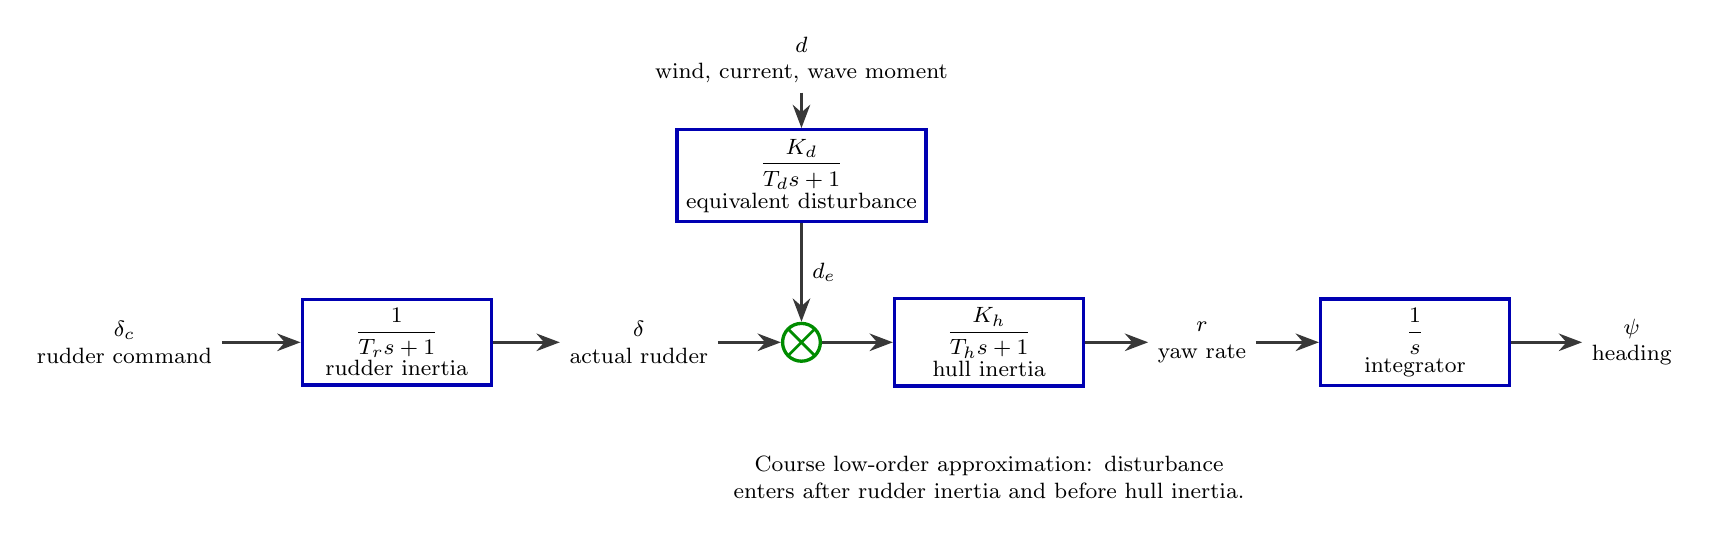
\begin{tikzpicture}[
  >=Stealth,
  signal/.style={->, line width=1.2pt, draw=black!78},
  block/.style={
    rectangle,
    draw=blue!70!black,
    line width=1.2pt,
    minimum width=2.4cm,
    minimum height=1.0cm,
    align=center,
    font=\footnotesize
  },
  sum/.style={
    circle,
    draw=green!55!black,
    line width=1.2pt,
    minimum size=0.48cm,
    inner sep=0pt,
    path picture={
      \draw[green!55!black,line width=1pt]
        (path picture bounding box.south west) -- (path picture bounding box.north east)
        (path picture bounding box.north west) -- (path picture bounding box.south east);
    }
  },
  labelbox/.style={font=\footnotesize, align=center}
]
  \node[labelbox] (cmd) at (0,0) {$\delta_c$\\rudder command};
  \node[block, right=1.0cm of cmd] (servo) {$\dfrac{1}{T_r s+1}$\\rudder inertia};
  \node[labelbox, right=0.85cm of servo] (actual) {$\delta$\\actual rudder};
  \node[sum, right=0.8cm of actual] (sumd) {};
  \node[block, right=0.9cm of sumd] (hull) {$\dfrac{K_h}{T_hs+1}$\\hull inertia};
  \node[labelbox, right=0.8cm of hull] (yaw) {$r$\\yaw rate};
  \node[block, right=0.8cm of yaw] (int) {$\dfrac{1}{s}$\\integrator};
  \node[labelbox, right=0.9cm of int] (heading) {$\psi$\\heading};

  \node[block, above=1.25cm of sumd] (dist) {$\dfrac{K_d}{T_d s+1}$\\equivalent disturbance};
  \node[labelbox, above=0.45cm of dist] (dlabel) {$d$\\wind, current, wave moment};

  \draw[signal] (cmd) -- (servo);
  \draw[signal] (servo) -- (actual);
  \draw[signal] (actual) -- (sumd);
  \draw[signal] (sumd) -- (hull);
  \draw[signal] (hull) -- (yaw);
  \draw[signal] (yaw) -- (int);
  \draw[signal] (int) -- (heading);
  \draw[signal] (dlabel) -- (dist);
  \draw[signal] (dist) -- node[right, font=\footnotesize] {$d_e$} (sumd);

  \node[font=\footnotesize, align=center, below=0.75cm of hull, text width=6.7cm]
    {Course low-order approximation: disturbance enters after rudder inertia and before hull inertia.};
\end{tikzpicture}
\end{document}
